\documentclass[tikz,border=10pt]{standalone}
\usepackage{tikz}
\usetikzlibrary{arrows.meta,positioning,shapes.geometric,decorations.pathreplacing}

\begin{document}
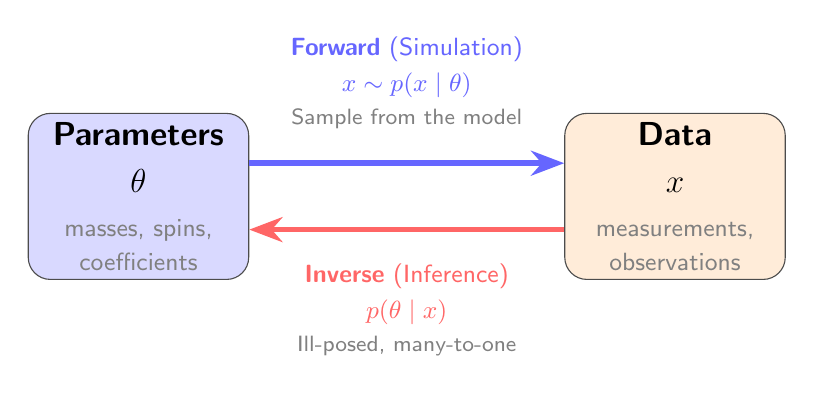
\begin{tikzpicture}[
    node distance=4cm,
    box/.style={
        rectangle,
        rounded corners=8pt,
        draw=black!70,
        fill=#1,
        minimum width=2.8cm,
        minimum height=1.8cm,
        align=center,
        font=\sffamily\large
    },
    arrow/.style={
        ->,
        >=Stealth,
        line width=2pt,
        #1
    },
    label/.style={
        font=\sffamily\small,
        align=center
    }
]

% Parameters box
\node[box=blue!15] (theta) {
    \textbf{Parameters}\\[3pt]
    $\theta$\\[2pt]
    {\small\color{gray}masses, spins,}\\[-2pt]
    {\small\color{gray}coefficients}
};

% Data box
\node[box=orange!15, right=of theta] (x) {
    \textbf{Data}\\[3pt]
    $x$\\[2pt]
    {\small\color{gray}measurements,}\\[-2pt]
    {\small\color{gray}observations}
};

% Forward arrow (top)
\draw[arrow=blue!60] ([yshift=12pt]theta.east) -- ([yshift=12pt]x.west)
    node[midway, above=8pt, label] {
        \textbf{Forward} (Simulation)\\[2pt]
        $x \sim p(x \mid \theta)$\\[1pt]
        {\footnotesize\color{gray}Sample from the model}
    };

% Inverse arrow (bottom)
\draw[arrow=red!60] ([yshift=-12pt]x.west) -- ([yshift=-12pt]theta.east)
    node[midway, below=8pt, label] {
        \textbf{Inverse} (Inference)\\[2pt]
        $p(\theta \mid x)$\\[1pt]
        {\footnotesize\color{gray}Ill-posed, many-to-one}
    };

\end{tikzpicture}
\end{document}
